% ---- pg-115 （书页 103） ----

改变剩余向量的比例, 相当于对每一个原始的观测值 $x_{ik}$ 用它的标准化值 $(x_{ik}-\bar{x}_{k})/\sqrt{s_{kk}}$ 替换. 标准化变量的样本协方差矩阵就是 $\mathbf{R}$, 即原始变量的样本相关阵(参考练习 3.13). 我们定义
\begin{mvbox}
\phantomsection\label{eq:3-19}
\begin{equation}
(\text{标准化变量的广义样本方差})=|\mathbf{R}| \tag{3-19}
\end{equation}
\end{mvbox}
由于所得到的向量
\[
[(x_{1k}-\bar{x}_{k})/\sqrt{s_{kk}},(x_{2k}-\bar{x}_{k})/\sqrt{s_{kk}},\cdots,(x_{nk}-\bar{x}_{k})/\sqrt{s_{kk}}]=(\mathbf{y}_{k}-\bar{x}_{k}\mathbf{1})'/\sqrt{s_{kk}}
\]
的长度都为 $\sqrt{n-1}$, 当这些向量几乎正交时, 标准化变量的广义样本方差较大, 而当这些向量的两个或更多个几乎是同一方向时, 广义样本方差较小. 利用推导出\hyperref[eq:3-7]{式(3-7)}的方法, 容易求出 $(\mathbf{y}_{i}-\bar{x}_{i}\mathbf{1})/\sqrt{s_{ii}}$ 和 $(\mathbf{y}_{k}-\bar{x}_{k}\mathbf{1})/\sqrt{s_{kk}}$ 之间夹角 $\theta_{ik}$ 的余弦是样本相关系数 $r_{ik}$. 因此, 我们可以作出结论: 当所有 $r_{ik}$ 接近零时, $|\mathbf{R}|$ 较大, 而当 $r_{ik}$ 中一个或多个是接近 1 或 $-1$ 时, $|\mathbf{R}|$ 较小.

总而言之, 有如下结论: 设
\[
\frac{(\mathbf{y}_{i}-\bar{x}_{i}\mathbf{1})}{\sqrt{s_{ii}}}=\begin{bmatrix}\dfrac{x_{1i}-\bar{x}_{i}}{\sqrt{s_{ii}}}\\\dfrac{x_{2i}-\bar{x}_{i}}{\sqrt{s_{ii}}}\\\vdots\\\dfrac{x_{ni}-\bar{x}_{i}}{\sqrt{s_{ii}}}\end{bmatrix},\quad i=1,2,\cdots,p
\]
是标准化变量的偏差向量. 这些偏差向量在 $\mathbf{d}_{i}$ 的方向上, 而长度平方为 $n-1$. 在 $p$ 维空间中由偏差向量生成的体积, 与广义样本方差有关. 采用与推导\hyperref[eq:3-15]{式(3-15)}同样的步骤, 有:
\phantomsection\label{eq:3-20}
\begin{equation}
\left(\begin{matrix}\text{标准化变量的}\\\text{广义样本方差}\end{matrix}\right)=|\mathbf{R}|=(n-1)^{-p}(\text{体积})^{2} \tag{3-20}
\end{equation}

对于\hyperref[fig:3.6]{图 3.6} 中的偏差向量, 标准化变量的偏差向量所形成的体积, 如\hyperref[fig:3.10]{图 3.10} 所示. 比较\hyperref[fig:3.10]{图 3.10} 与\hyperref[fig:3.6]{图 3.6}, 显示出 $\mathbf{d}_{2}$ 向量(在 $x_{2}$ 上较大的变化性)对体积平方 $|\mathbf{S}|$ 的影响比它对体积平方 $|\mathbf{R}|$ 的影响大得多.

\begin{mvfigure}
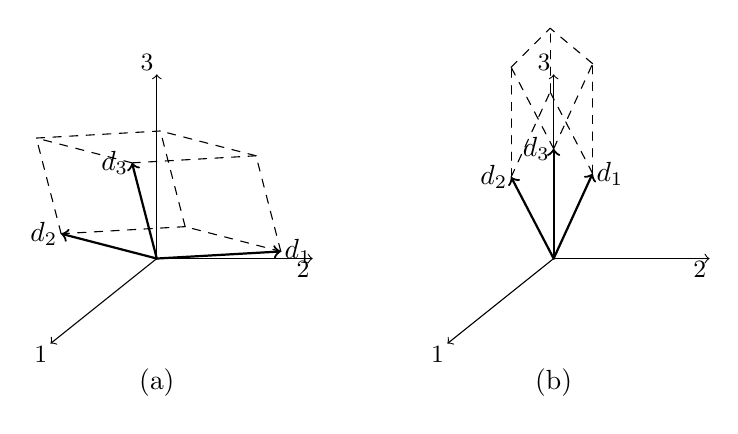
\begin{tikzpicture}[scale=0.9,line join=round,line cap=round]
% ---------- (a) 原偏差向量 ----------
\begin{scope}
\draw[->] (0,0) -- (2.20,0) node[below left,inner sep=1pt,font=\small] {2};
\draw[->] (0,0) -- (0,2.60) node[above left,inner sep=1pt,font=\small] {3};
\draw[->] (0,0) -- (-1.50,-1.20) node[below left,inner sep=1pt,font=\small] {1};
\draw[->,thick] (0,0) -- (1.75,0.10) node[right,inner sep=1pt] {$d_{1}$};
\draw[->,thick] (0,0) -- (-1.35,0.35) node[left,inner sep=1pt] {$d_{2}$};
\draw[->,thick] (0,0) -- (-0.35,1.35) node[left,inner sep=1pt] {$d_{3}$};
% 平行六面体（虚线）
\draw[dashed] (1.75,0.10) -- (0.40,0.45);
\draw[dashed] (-1.35,0.35) -- (0.40,0.45);
\draw[dashed] (1.75,0.10) -- (1.40,1.45);
\draw[dashed] (-0.35,1.35) -- (1.40,1.45);
\draw[dashed] (-1.35,0.35) -- (-1.70,1.70);
\draw[dashed] (-0.35,1.35) -- (-1.70,1.70);
\draw[dashed] (0.40,0.45) -- (0.05,1.80);
\draw[dashed] (1.40,1.45) -- (0.05,1.80);
\draw[dashed] (-1.70,1.70) -- (0.05,1.80);
\node at (0,-1.75) {(a)};
\end{scope}
% ---------- (b) 标准化偏差向量 ----------
\begin{scope}[xshift=5.6cm]
\draw[->] (0,0) -- (2.20,0) node[below left,inner sep=1pt,font=\small] {2};
\draw[->] (0,0) -- (0,2.60) node[above left,inner sep=1pt,font=\small] {3};
\draw[->] (0,0) -- (-1.50,-1.20) node[below left,inner sep=1pt,font=\small] {1};
\draw[->,thick] (0,0) -- (0.55,1.20) node[right,inner sep=1pt] {$d_{1}$};
\draw[->,thick] (0,0) -- (-0.60,1.15) node[left,inner sep=1pt] {$d_{2}$};
\draw[->,thick] (0,0) -- (0.00,1.55) node[left,inner sep=1pt] {$d_{3}$};
% 平行六面体（虚线）
\draw[dashed] (0.55,1.20) -- (-0.05,2.35);
\draw[dashed] (-0.60,1.15) -- (-0.05,2.35);
\draw[dashed] (0.55,1.20) -- (0.55,2.75);
\draw[dashed] (0.00,1.55) -- (0.55,2.75);
\draw[dashed] (-0.60,1.15) -- (-0.60,2.70);
\draw[dashed] (0.00,1.55) -- (-0.60,2.70);
\draw[dashed] (-0.05,2.35) -- (-0.05,3.25);
\draw[dashed] (0.55,2.75) -- (-0.05,3.25);
\draw[dashed] (-0.60,2.70) -- (-0.05,3.25);
\node at (0,-1.75) {(b)};
\end{scope}
\end{tikzpicture}
\phantomsection\label{fig:3.10}\mvcap{图 3.10\quad 由标准化变量的等长度偏差向量生成的体积}
\end{mvfigure}
